\section{Architecture}

The main application is divided into three modules.
Two additional modules serve to test the agent and document the application.
These modules are briefly summarised in Table \ref{tab:modules}, and their interactions are illustrated in Figure \ref{fig:architecture}.

\begin{table}[h]
\centering
\begin{tabular}{|l|p{10cm}|}
\hline
\textbf{Module} & \textbf{Primary purpose} \\
\hline
\textbf{Frontend} & Desktop application that the user interacts with. \\
\hline
\textbf{Sidecar} & Manages local file operations and tools for the agent. \\
\hline
\textbf{Agent} & Server that runs the AI agent and orchestrates agentic operations. \\
\hline
\textbf{User guide} & Documentation for users to install and use the application. \\
\hline
\textbf{Benchmark} & Tool for evaluating agent and LLM performance on the test dataset. \\
\hline
\end{tabular}
\caption{Modules of the Spartan Write system}
\label{tab:modules}
\end{table}

\begin{figure}[htbp]
\centering
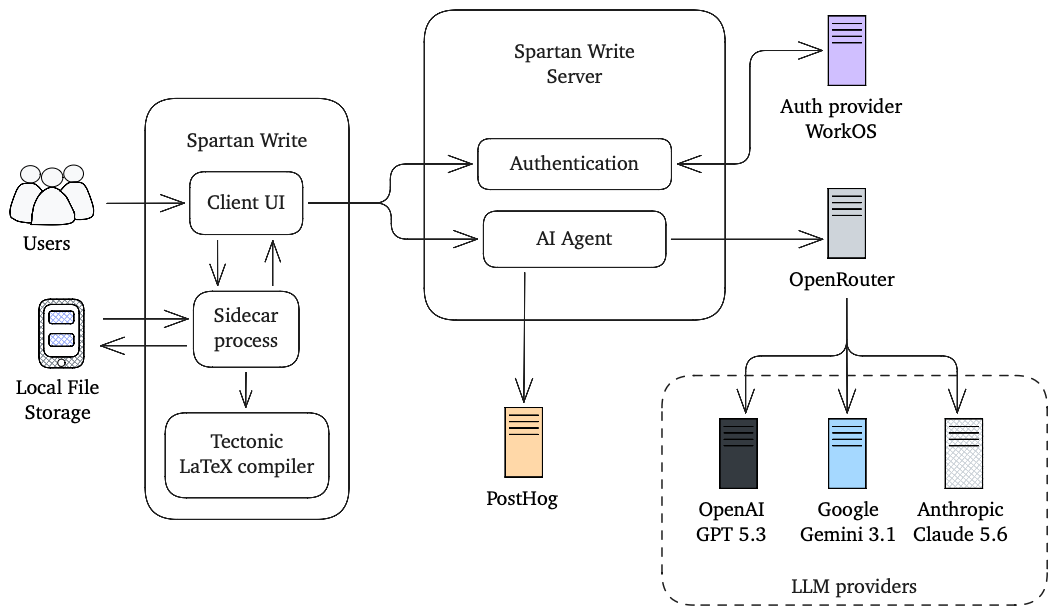
\includegraphics[width=1\linewidth]{figures/architecture.excalidraw.png}
\caption{Spartan Write system architecture}
\label{fig:architecture}
\end{figure}

\subsection{Frontend}

Spartan Write's frontend is built with React.js \cite{react} on Tauri, enabling cross-platform development of native desktop applications for macOS, Windows, and Linux from a single TypeScript/React codebase \cite{tauri}.

Accessibility is a core design principle in Spartan Write.
It includes configurable text zoom and a magnifier.
It also has support for screen readers.
The UI is built with industry-standard components designed with accessibility in mind.

\subsubsection{Development tooling and libraries}

\begin{itemize}
    \item Tauri provides wrappers for native system APIs while minimising binary size \cite{tauri}.
    This facilitates deploying to all major OSs using a single codebase.
    \item Vite powers fast build times and hot module reloading during development \cite{vite}.
    \item TypeScript provides type safety and is the industry standard \cite{typescript}.
    \item Styling is handled by Tailwind CSS for responsive, utility-first design \cite{tailwind}.
    \item User interface components are derived from shadcn, a UI component library built with accessibility and consistent visual design in mind \cite{shadcn}.
    \item The source code editor implements the Monaco Editor which provides syntax highlights \cite{monaco}.
\end{itemize}

\subsubsection{Authentication}

The frontend integrates WorkOS AuthKit to provide secure, standards-based authentication \cite{workos}.
The authentication framework follows best practices for security and developer and user convenience.
Once authenticated, the frontend manages user credentials and conveys usage data.
Only authenticated users are permitted to invoke the agent.

\subsubsection{Project management}

The frontend provides a dashboard to view and open recent projects.
There is an onboarding flow for new users and a settings page that displays user profile information and usage analytics.

\subsubsection{Editor}

The editor features a resizable layout that supports two modes.
In \emph{source view}, users see a \LaTeX\ code editor.
In \emph{preview view}, which is the default, users see a live PDF render of their document.
The chat interface is available in both views.
This design allows users to see the changes made by the agent as they occur.

\subsection{Sidecar}

The sidecar is a local FastAPI server \cite{fastapi} bundled with the desktop application that serves as the bridge between the frontend UI and the project filesystem.
Unlike most "servers", this program runs on the users' devices alongside the client application \cite{tauri_sidecar}.
Its primary responsibility is to handle all local filesystem operations.
This keeps the cloud server stateless and focused purely on AI agent logic.

The sidecar also manages project-specific and user-level configuration, including user information, API credentials in case the user is able to provide their own API key, and authentication tokens.
These settings are persisted locally for quick access and offline operation.
The sidecar encapsulates all local, filesystem-bound operations, compilation, and configuration management.

\subsubsection{Template discovery}

The sidecar provides an endpoint that lists available project templates, enabling the frontend to present users with choices when creating new projects.
This allows for easy extensibility: new templates can be added to the sidecar without requiring frontend changes.

\subsubsection{Compilation and PDF rendering}

A critical function of the sidecar is local \LaTeX\ compilation.
For this purpose, it uses Tectonic \cite{tectonic}, a lightweight \LaTeX\ compiler to compile the project.
The sidecar abstracts this program behind a convenient API that returns the compilation status and error messages to the frontend.
The compiled PDF is served back to the frontend for live preview.
The Tectonic binary is bundled alongside the sidecar itself as part of the frontend application \cite{tauri_sidecar}.
This local compilation strategy facilitates fast iteration cycles without reliance on cloud-based typesetting services.


\subsubsection{Agentic AI chat integration}

The frontend integrates CopilotKit which facilitates a fully featured agentic chat interface \cite{copilotkit}.
The sidecar is equipped with tools for the agent to perform comprehensive document manipulation: reading, writing, deleting, and renaming files; listing project contents; compiling \LaTeX\; and forwarding errors, if any; and managing attached images.
All file operations include path validation to prevent traversal attacks and ensure modifications remain within the project directory.
This toolset allows the agent to make changes to the project files and update the document to satisfy the user's request.

\subsubsection{Image processing}

There are two ways that the agent may choose to handle images.
Based on the user's request, the agent may decide that the image must be included in the document or processed to answer a question or make a decision.
In the first case, the agent need not process the image at all, and would simply need a tool to copy it into the project directory.
Then, it could generate code to render the image within the document.
In the second case, the image would not need to be copied or stored.
Instead, it would be processed by the agent.
The sidecar provides tools for both of these purposes.

\subsection{Agent}

The Agent is the cloud-based AI backbone of Spartan Write.
It is responsible for interpreting user requests and orchestrating intelligent document edits.
It is built on Python FastAPI \cite{fastapi}.
The agent's behaviour is defined using LangGraph, a framework for building stateful, multi-step AI workflows that maintain conversation context and carry out complex editing logic deterministically \cite{langgraph}.
It validates all user actions through WorkOS authentication \cite{workos} and streams the generated response to the frontend.
Rather than being locked to a single provider, the agent integrates with OpenRouter.
OpenRouter is a configurable LLM aggregation layer that allows selection from multiple language models and providers \cite{openrouter}.
LLM usage is reported to PostHog \cite{posthog}.

\subsubsection{Cloud deployment}

The agent is containerised and deployed to a virtual machine on the cloud.
Its stateless architecture ensures that no persistent state is maintained between requests.
It also enables independent scaling across multiple instances.

\subsubsection{Analytics \& privacy}

Every agent interaction is tracked and reported to PostHog for usage analytics, billing, and performance insights \cite{posthog}.
Conversation history is maintained within a single session to support multi-turn coherence. To protect privacy, chats are not persisted across separate chats.

\subsection{Benchmark}

The benchmark systematically assesses the agent's performance in various document editing scenarios.
It executes the test dataset against the agent API and applies multi-faceted scoring metrics.
This provides data-backed insights into agent capabilities, identifies performance bottlenecks, and enables comparisons across different models and configurations.
The goal is to select the most feasible language model and to evaluate the changes in performance as the models update.

\subsubsection{Testing workflow}

The benchmark uses a curated set of document states paired with pre-defined user prompts. 
Each dataset item represents a specific editing task.
This evaluates the agent's capabilities across a range of real-world scenarios.

The benchmark directly interacts with the agent server via its REST API.
It sends test prompts, captures agent responses and tool invocations, and stores the results in a database.

\subsubsection{Reproducibility}

By maintaining the test dataset and deterministic scoring logic, the benchmark enables reproducible testing across configurations.
This is essential for making an informed decision.
The standardised evaluation approach also supports tracking improvements or regressions over time as the agent/model evolves.

\subsubsection{Visualisation}

Results are visualised using Plotly \cite{plotly} on a Streamlit-based web dashboard \cite{streamlit}.
The dashboard presents evaluation results using various aggregations that are discussed in the coming sections.
This interactive interface supports the identification of performance shifts and failure modes and enables comparative analysis across different models.

\subsection{User guide}

The user guide is built a lightweight documentation framework called MkDocs.
It generates a clean searchable website from Markdown files.

The guide is hosts user-facing documentation across all platforms, with built-in search functionality, responsive design, and clear navigation.
It covers the complete user journey, from platform-specific installation instructions for macOS, Windows, and Linux, to quick-start tutorials for first-time users, and to comprehensive reference material on project management, API configuration, tips for efficient agent usage, best practices, and troubleshooting.
This breadth of content ensures users can find answers at every stage of their experience with Spartan Write.
